%%%%%%%%%%%%%%%%%%%%%%%%%%%%%%%%%%%%%%%%%%%%
\section{Conclusiones y trabajo futuro}

\begin{frame}
      \frametitle{Contenido}
      \tableofcontents[currentsection]
\end{frame}

%%%%%%%%%%%%%%%%%%%%%%%%%%%%%%%%%%%%%%%%%%%%%%%%%%%%%%%%
{
%\paper{Lastname N. YEAR in journal of...}
\begin{frame}{Conclusiones y trabajo futuro}

  \begin{columns}
  \begin{column}{.75\linewidth}

  \textbf{Conclusiones}   

  \begin{itemize}
    %\item Applied Montessory Education and spiral education to design child-based curriculumns in AI and Robotics
    \item Se aplico el m\'etodo Montessory y m\'etodo espiral para dise\~nar curriculms de IA y Rob\'otica para ni\~nos
    %\item Piloted a workshop with 14 participants of 4 lessons surveying attitudes with liker chart
    \item Se piloteo un taller con un curriculum de 4 lecciones, con 14 participantes, evaluando resultados de actitudes de ingenier\'ia y ciencia usando Wilcoxon and escala liker 
  \end{itemize}

  \textbf{Trabajo futuro}
  \begin{itemize}
    \item Mejorar las encuetas y el anal\'isis estad\'istico 
    \item Pilotear el taller con un major n\'umero de participantes
    \item Aplicar a esquemas de financiamiento
    \item Iniciar relaciones legisladores internaciones que promuevan el proyecto air4children
\end{itemize}

    \end{column}


  \begin{column}{.3\linewidth}

      \begin{figure}
        \centering
        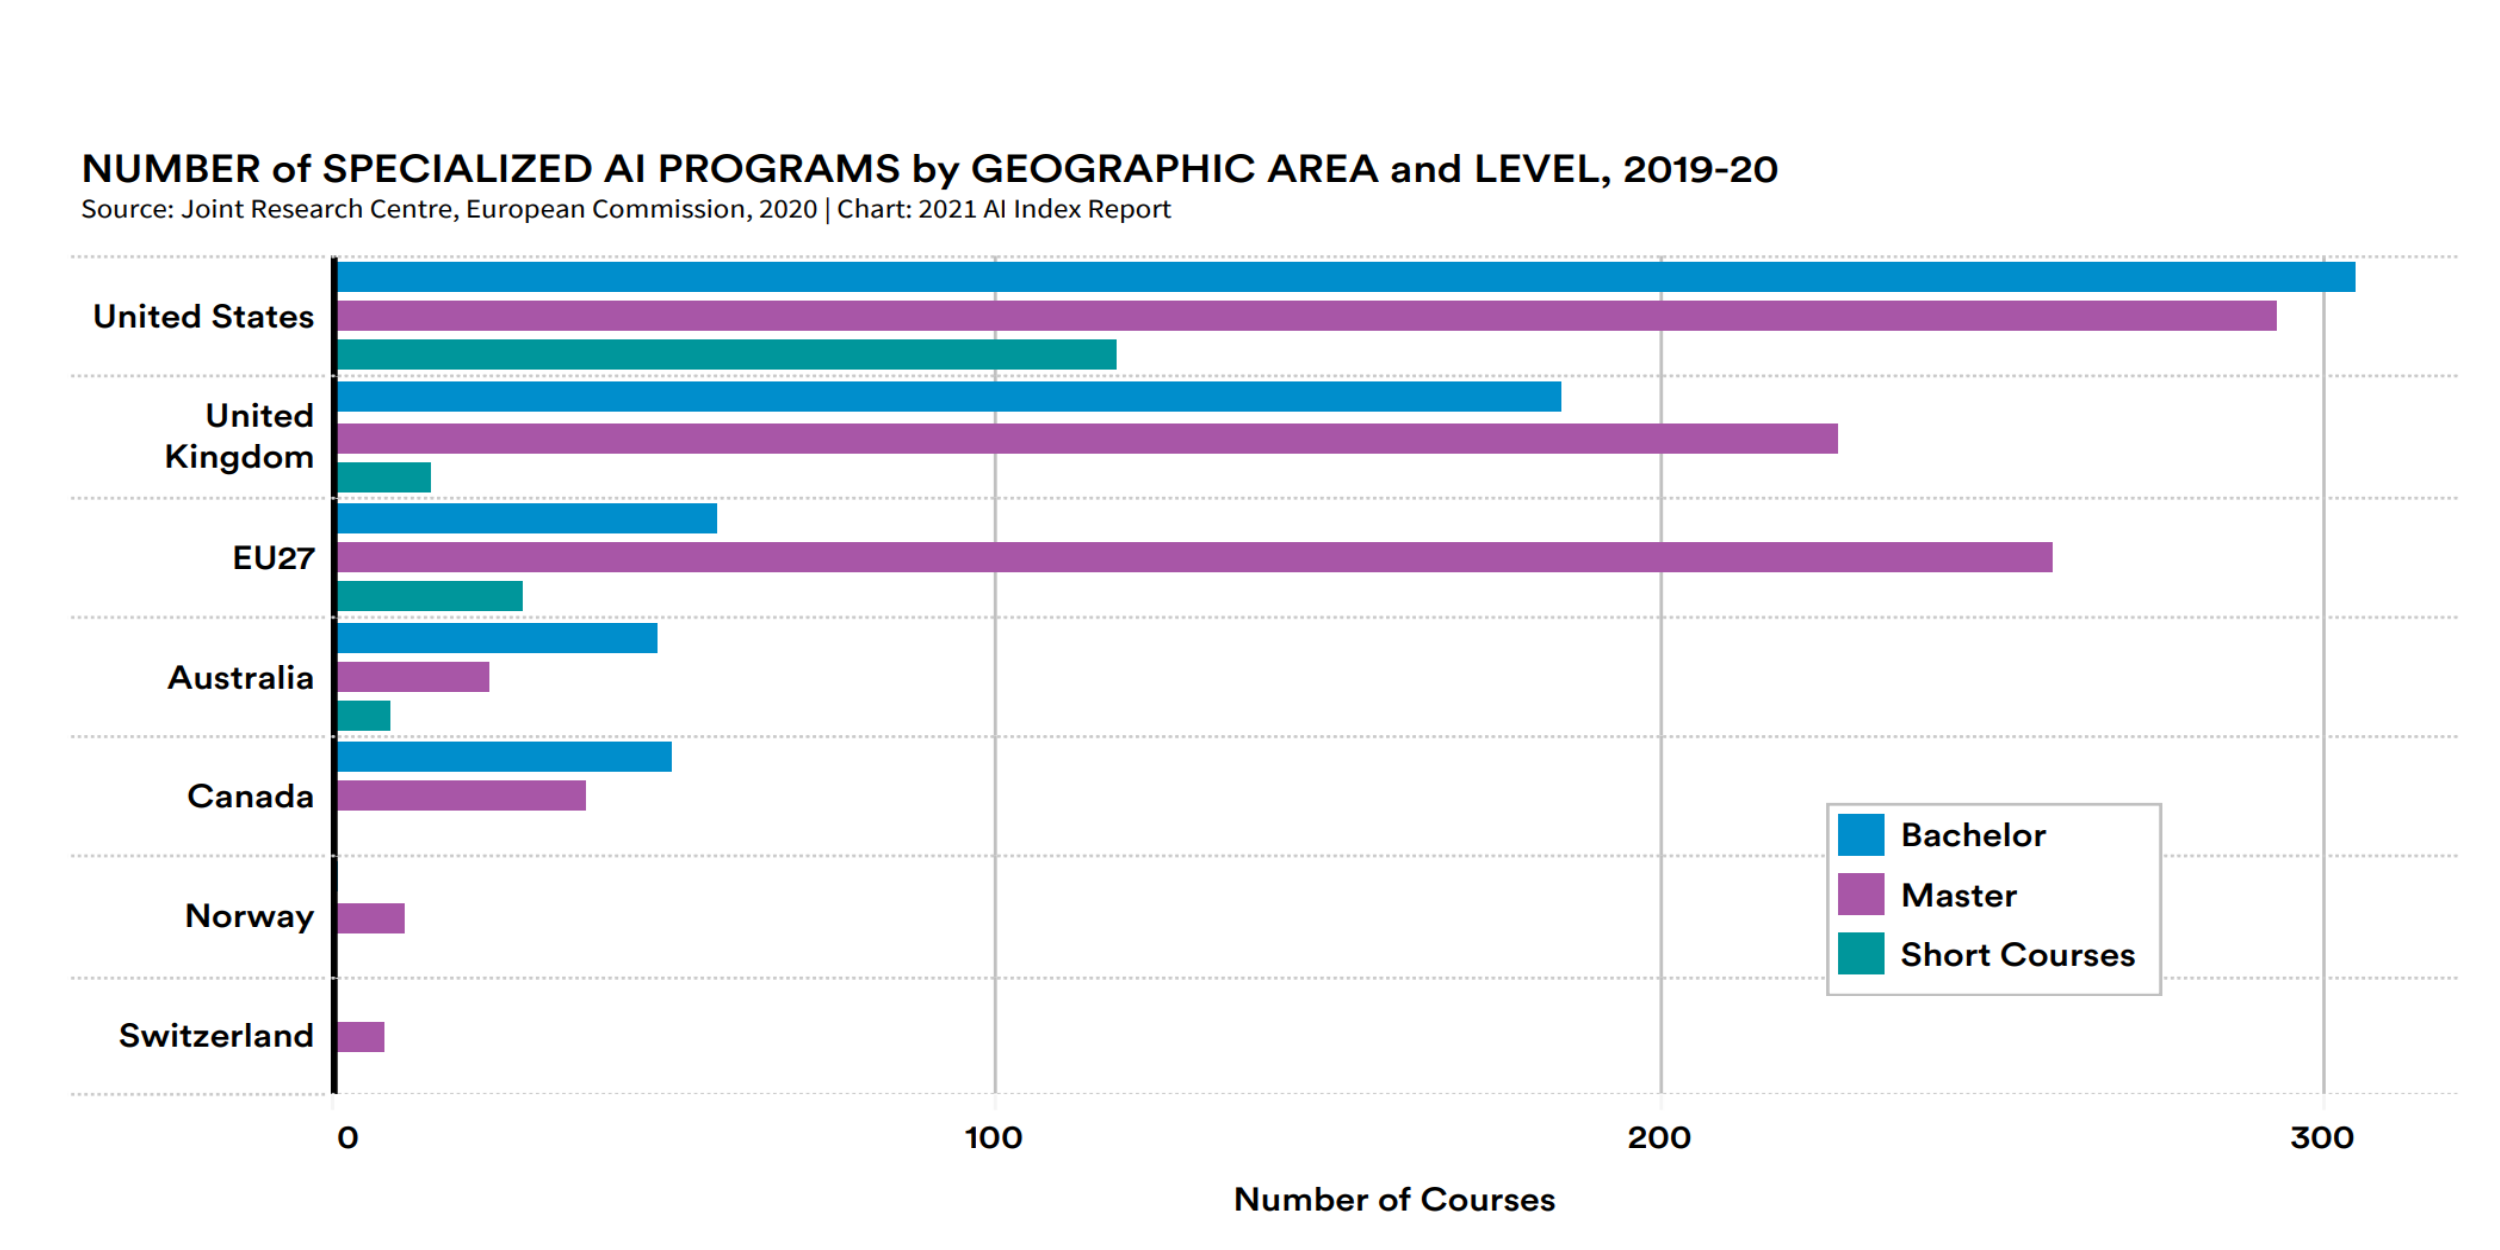
\includegraphics[width=0.9\textwidth]{./logo/outputs/drawing-v00.png}
      \end{figure}

    \end{column}
  \end{columns}

\end{frame}
}


%%%%%%%%%%%%%%%%%%%%%%%%%%%%%%%%%%%%%%%%%%%%%%%%%%%%%%%%%
%{
%%\paper{Lastname N. YEAR in journal of...}
%\begin{frame}{Acknowledgements}
%
%  \begin{figure}
%  \centering
%  
\includegraphics[width=1.0\textwidth]{./figures/team/outputs/drawing-v00.png}
%  \end{figure}
%
%\end{frame}
%}
%
